A physical anthropologist performed a mineral analysis of nine ancient Peruvian hairs.
The results for the chromium ($x_{1}$) and strontium ($x_{2}$) levels,in parts per million (ppm),
were as follows:

\begin{center}
    \begin{NiceTabular}{c|ccccccccc}
        \hline
        \addlinespace[0.1cm]
        $x_{1}\text{(Cr)}$ & .48 & 40.53 & 2.19 & .55 & .74 & .66 & .93 & .37 & .22 \\
        \addlinespace[0.1cm]
        \hline
        \addlinespace[0.1cm]
        $x_{2}\text{(St)}$ & 12.57 & 73.68 & 11.13 & 20.03 & 20.29 & .78 & 4.64 & .43 & 1.08 \\
        \addlinespace[0.1cm]
        \hline
        \Block[l]{1-10}{\footnotesize{Source: Benfer and others, ``Mineral Analysis of Ancient Peruvian Hair,'' \textit{American}} \\
        \addlinespace[-0.1cm]
        \footnotesize{\textit{Journal of Physical Anthropology}, \textbf{48}, no. 3 (1978), 277-282.}}
    \end{NiceTabular}
\end{center}

It is known that low levels (less than or equal to .100 ppm) of chromium suggest the
presence of diabetes, while strontium is an indication of animal protein intake.

\begin{enumerate}[label=(\alph*)]
    \item Construct and plot a 90\% joint confidence ellipse for the population mean vector
    $\bm{\mu} = [\mu_{1} , \mu_{2}]$, assuming that these nine Peruvian hairs represent a random sample
    from individuals belonging to a particular ancient Peruvian culture.

    \begin{figure}[H]
        \centering
            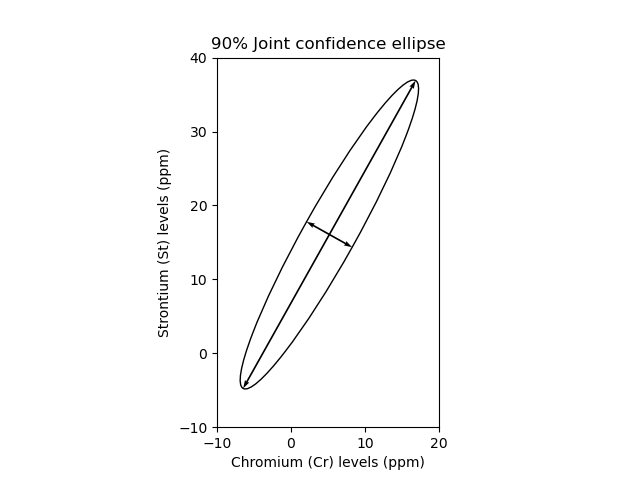
\includegraphics[scale=0.75]{./python/chapter-5/Question-5-11-a.png}
    \end{figure}

    \item Obtain the individual simultaneous 90\% confidence intervals for $\mu_{1}$ and $\mu_{2}$ by ``projecting''
    the ellipse constructed in Part a on each coordinate axis. (Alternatively, we
    could use Result 5.3.) Does it appear as if this Peruvian culture has a mean strontium
    level of 10? That is, are any of the points ($\mu_{2}$ arbitrary, 10) in the confidence regions?
    Is ${[.30, 10]}^{\prime}$ a plausible value for $\bm{\mu}$? Discuss.
    \newline
    \par
    Yeah, we could just use Result 5.3, but I'll take the long road.
    From the top of page 259, it says, ``the projection of the ellipsoid on $\textbf{u}$ is $c\sqrt{\textbf{u}^{\prime}\textbf{A}\textbf{u}}\textbf{u}/\textbf{u}^{\prime}\textbf{u}$ and it's length is $c\sqrt{\textbf{u}^{\prime}\textbf{A}\textbf{u}/\textbf{u}^{\prime}\textbf{u}}$. With the unit vector $\textbf{e}_{\textbf{u}} = \textbf{u}/\|\textbf{u}\|$ the projection extends
    \[
        \sqrt{
            c^{2}
            \textbf{e}_{\textbf{u}}^{\prime}
            \textbf{A}
            \textbf{e}_{\textbf{u}}
            }
            =
            \frac{c}{\|\textbf{u}\|}
            \sqrt{\textbf{u}^{\prime}\textbf{A}\textbf{u}}
            \text{ units along }\textbf{u}
    \]
    The projection of the ellipsoid also extends the same length in the direction of $-\textbf{u}$''.

    So from this, if we pick $\textbf{u} = \textbf{a}$, where $\textbf{a}^{\prime} = [0, \dots, 0, a_{i}, 0, \dots, 0]$ and $a_{i} = 1$. And $\textbf{A} = (1/n)\textbf{S}$, we have
    \[
        \|\textbf{a}\|
        =
        \sqrt{0^{2} + \dots + 1^{2} + 0^{2} + \dots + 0^{2}}
        =
        \sqrt{1}
        =
        1
    \]
    so the length of the projection is
    \[
        c
        \sqrt{
            \frac{
                \textbf{u}^{\prime}
                \textbf{A}
                \textbf{u}
            }{
                \textbf{u}^{\prime}\textbf{u}
            }
        }
        =
        \frac{c}{\|\textbf{u}\|}
        \sqrt{\textbf{u}^{\prime}\textbf{A}\textbf{u}}
        =
        \frac{c}{\|\textbf{a}\|}
        \sqrt{
            \textbf{a}^{\prime}
            \left(\textbf{S}/n\right)
            \textbf{a}
            }
        =
        \frac{c}{1}
        \sqrt{
            \frac{
                \textbf{a}^{\prime}
                \textbf{S}
                \textbf{a}
            }{n}
            }
        =
        c
        \sqrt{
            \frac{
                \textbf{a}^{\prime}
                \textbf{S}
                \textbf{a}
            }{n}
            }
    \]
    The vectors don't start at the origin, $\textbf{0}$, they start at $\textbf{a}^{\prime}\bar{\textbf{x}}$, and they go in both positive and negative directions, so we can add and subtract what's above (the length of the projection) from $\textbf{a}^{\prime}\bar{\textbf{x}}$ and we now have
    \[
        \textbf{a}^{\prime}\bar{\textbf{x}}
        \pm
        c
        \sqrt{
            \frac{
                \textbf{a}^{\prime}
                \textbf{S}
                \textbf{a}
            }{n}
            }
    \]
    Finally, we know that $c = \sqrt{\frac{(n-1)p}{(n-p)}F_{p, n-p}(\alpha)}$, and plugging that in we have
\[
        \textbf{a}^{\prime}\bar{\textbf{x}}
        \pm
        c
        \sqrt{
            \frac{(n-1)p}{(n-p)}F_{p, n-p}(\alpha)
            \frac{
                \textbf{a}^{\prime}
                \textbf{S}
                \textbf{a}
            }{n}
            }
    \]
    Well ring a ding ding, this is the same as Result 5.3.

    \[
        \bar{\textbf{x}}
        =
        \begin{bNiceArray}{c}
             5.1856 \\
            16.0700
        \end{bNiceArray},
        \hspace{0.4cm}
        \textbf{S}
        =
        \begin{bNiceArray}{rr}
            176.0042 & 287.2412 \\
            287.2412 & 527.8493
        \end{bNiceArray}
    \]

    \[
        \begin{NiceArray}{rrrr}
            5.19 \pm \sqrt{7.45} \frac{\sqrt{176.00}}{\sqrt{9}} & \text{contains }\mu_{1} & \text{ or } & -6.88 \leq \mu_{1} \leq 17.25 \\
            16.07 \pm \sqrt{7.45} \frac{\sqrt{527.85}}{\sqrt{9}} & \text{contains }\mu_{2} & \text{ or } & -4.83 \leq \mu_{2} \leq 36.97
        \end{NiceArray}
    \]
    The value of 10 is within the CI for St ($\mu_{2}$), so we would fail to reject the null hypothesis that $\mu_{2} = 10$. The value of ${[.30, 10]}^{\prime}$ is a plausible value for $\bm{\mu}$, since it's within our simultaneous confidence ellipse as seen below.

    \begin{figure}[H]
        \centering
            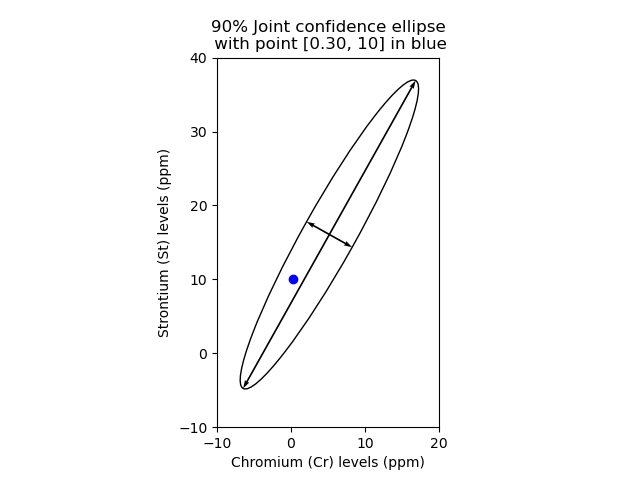
\includegraphics[scale=0.75]{./python/chapter-5/Question-5-11-b.png}
    \end{figure}

    \item Do these data appear to be bivariate normal? Discuss their status with reference to
    Q-Q plots and a scatter diagram. If the data are not bivariate normal, what implications
    does this have for the results in Parts a and b?
    
    \begin{figure}[H]
        \centering
        \begin{tabular}{c}
            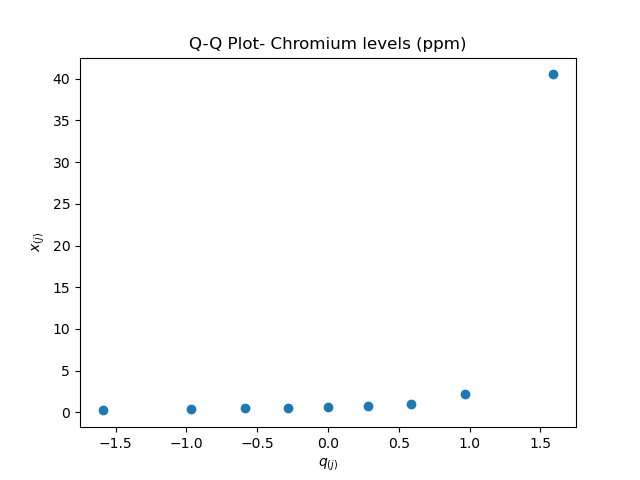
\includegraphics[scale=0.75]{./python/chapter-5/Question-5-11-c-QQ-Cr.png} \\
            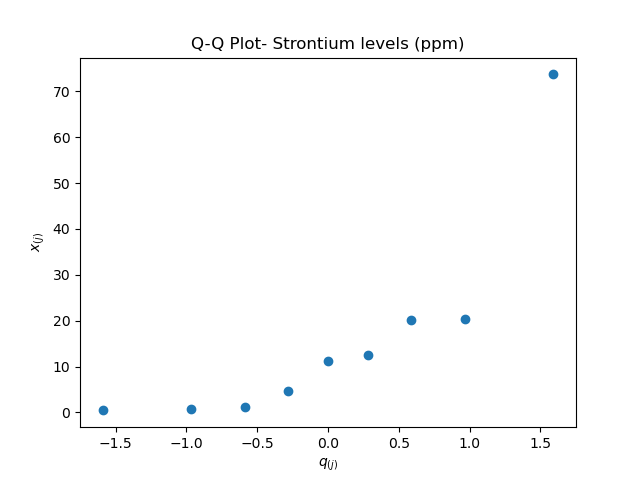
\includegraphics[scale=0.75]{./python/chapter-5/Question-5-11-c-QQ-St.png}
        \end{tabular}
    \end{figure}

    Both Q-Q plots do not appear to be normally distributed. Observation 2, has much larger Cr and St values than the other observations. The confidence ellipse is much larger and the confidence intervals we created in part (b) are much wider (and include negative values) than they would be without including the observation.

    \item Repeat the analysis with the obvious ``outlying'' observation removed. Do the inferences
    change? Comment.
    \begin{figure}[H]
        \centering
        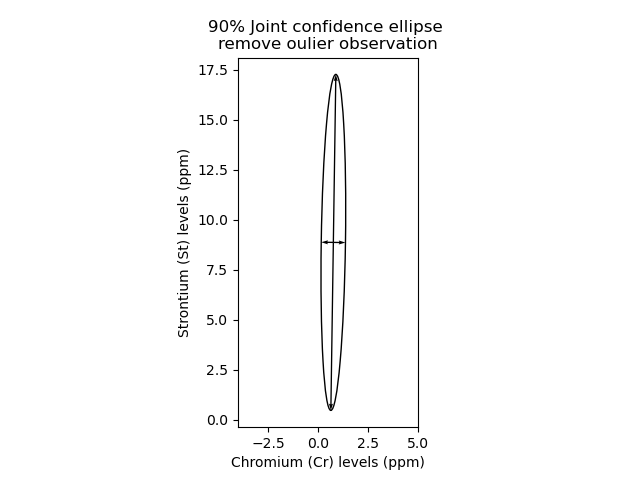
\includegraphics[scale=0.75]{./python/chapter-5/Question-5-11-d-CI-Ellipse.png}
    \end{figure}

    \begin{figure}[H]
        \centering
        \begin{tabular}{cc}
            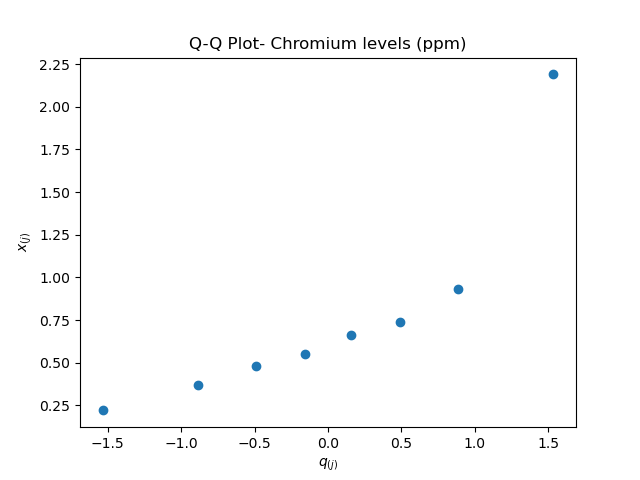
\includegraphics[scale=0.35]{./python/chapter-5/Question-5-11-d-QQ-Cr.png} &
            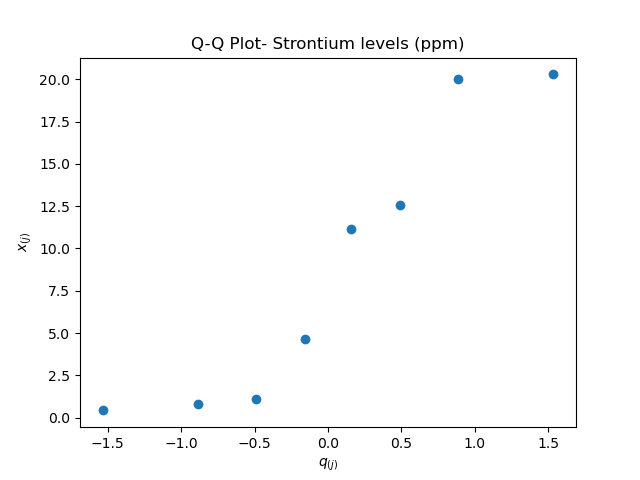
\includegraphics[scale=0.35]{./python/chapter-5/Question-5-11-d-QQ-St.png}
        \end{tabular}
    \end{figure}

    After deleting the outlier observation, the confidence ellipse shrinks and becomes almost vertical. The correlation coefficient between Cr and St also falls massively from 0.94 to 0.20. The 90\% simultaneous confidence intervals look a bit more reasonable, that is, not less than zero, with values of:

\[
        \begin{NiceArray}{rrrr}
            0.77 \pm \sqrt{8.08} \frac{\sqrt{0.38}}{\sqrt{8}} & \text{contains }\mu_{1} & \text{ or } & 0.15 \leq \mu_{1} \leq 1.39 \\
            8.87 \pm \sqrt{8.08} \frac{\sqrt{69.86}}{\sqrt{8}} & \text{contains }\mu_{2} & \text{ or } & 0.47 \leq \mu_{2} \leq 17.27
        \end{NiceArray}
    \]

    The Q-Q plot for Chromium still doesn't look very good after deleting the outlier. The Q-Q plot for Strontium has improved though. 

\end{enumerate}